\documentclass[10pt,twocolumn,letterpaper]{article}
\usepackage[pagenumbers]{cvpr}
\usepackage{multirow}
\definecolor{cvprblue}{rgb}{0.21,0.49,0.74}
\usepackage[breaklinks,colorlinks,allcolors=cvprblue]{hyperref}
\makeatletter\let\inputrows\@@input\makeatother
\def\confName{CS 412}
\def\confYear{2026}
\newcommand{\INFMIN}{0.914}
\newcommand{\INFMAX}{0.995}
\newcommand{\CROSSMAX}{0.460}
\newcommand{\CROSSMIN}{0.049}
\newcommand{\CROSSMAXAVG}{0.232}
\newcommand{\SPMLPMIN}{0.11}
\newcommand{\SPMLPMAX}{0.24}
\newcommand{\KSMED}{0.48}
\newcommand{\KSSHARE}{45}

\newcommand{\GITHUB}{\href{https://github.com/officialteekay/cs412-nids-generalization}{\nolinkurl{github.com/officialteekay/cs412-nids-generalization}}}

\newcommand{\ABSTRACT}{Machine learning intrusion detectors often report F1 scores above 0.95, but those scores usually come from training and testing on the same dataset. This project tests what happens when a detector trained on one network is moved to a different one. Logistic regression, a random forest, a multilayer perceptron, and a small self-attention model were trained on each of three NetFlow v2 datasets, UNSW-NB15, ToN-IoT, and CSE-CIC-IDS2018, and tested on all three. Every model scores between \INFMIN{} and \INFMAX{} F1 on its own network. On networks it was not trained on, its average F1 falls to between \CROSSMIN{} and \CROSSMAXAVG{}, which is below the 0.357 a detector gets by flagging every flow. The random forest is the best model in-dataset and the worst across networks, with an average cross-dataset AUC of 0.413. Training on two networks does not help with the third. The models rely on different features on each network, and in UNSW-NB15 a single rule on the TTL field reaches an F1 of 0.832 while flagging every flow on the other networks. Removing the TTL features does not fix transfer, because the models switch to other network-specific shortcuts.}

\newcommand{\ATTNCROSS}{The attention model, trained on the 60,000 flow subsample, reaches 0.232.}

\newcommand{\INTRORESULTS}{The results are clear. Every model looks strong in-dataset, with F1 between \INFMIN{} and \INFMAX{}. On networks they were not trained on, the average F1 of every model falls to between \CROSSMIN{} and \CROSSMAXAVG{}, which is lower than the 0.357 a detector gets by labeling every flow as an attack. The random forest is the best model in-dataset and the worst across networks, and its average cross-dataset AUC of 0.413 is below random guessing. The attention model gets a higher cross-dataset F1 than an MLP trained on the same data, but its AUC is the same and the extra F1 comes from flagging more flows. Training on two networks does not help with a third. The feature analysis shows that the models depend on different features on each network, and that a one-line rule on the TTL field reaches an F1 of 0.832 on UNSW-NB15. Removing the TTL features does not make the models transfer better.}

\newcommand{\ATTNPARA}{The self-attention model is the most complex model in this project, so it is the strongest test of this idea. It was trained on 60,000 flows per source, so the fair comparison is MLP-60k, which saw exactly the same training flows. Shrinking the training set barely changed the MLP. Its in-dataset F1 went from 0.968 to 0.964 and its cross-dataset F1 from 0.157 to 0.146, so the amount of training data is not what limits transfer.

Attention-60k has a higher average cross-dataset F1 than MLP-60k, 0.232 compared with 0.146, and its gap of 0.730 is the smallest of the five models. That looks like a real improvement at first, but the other numbers do not support it. Its average cross-dataset AUC is 0.496, almost the same as the 0.495 of MLP-60k, so it is no better at separating attacks from benign flows on a new network. Its cross-dataset false positive rate is higher, 0.398 compared with 0.322. Most of the F1 gain comes from the two cells where ToN-IoT is the test set. There, 64 percent of the flows are attacks, so a model that flags more flows gets a higher F1 almost automatically. The attention model also varies the most between seeds, with a standard deviation of 0.049 in its gap compared with 0.002 for MLP-60k. Overall, the attention model does not show a real advantage across networks.}

\newcommand{\FLAGPARA}{Table~\ref{tab:summary} also includes a trivial detector that labels every flow as an attack. Its F1 is not zero, because F1 depends on how common attacks are in the test set. It scores 0.077 on UNSW-NB15, 0.214 on CIC-IDS2018, and 0.780 on ToN-IoT, for an average of 0.357. Every trained model has a lower average cross-dataset F1 than this trivial detector. Cell by cell, logistic regression beats it in 2 of the 6 cross-dataset pairs, the MLP, MLP-60k, and attention model in 1 each, and the random forest in none. Flagging every flow is useless in practice because its false positive rate is 100 percent, but the comparison shows how little the cross-dataset F1 scores mean on their own.}

\newcommand{\MULTICAPTION}{Logistic regression, the random forest, and the MLP use three seeds. MLP-60k and Attention-60k use one seed and 30,000 flows from each source.}

\newcommand{\MULTIATTN}{MLP-60k, trained on the same flows as the attention model, goes from 0.146 to 0.134. The attention model is the only exception, going from 0.232 to 0.306. Most of that gain is on ToN-IoT, where it reaches 0.608, and its held-out AUC also rises to 0.663 on ToN-IoT and 0.806 on CIC-IDS2018. On CIC-IDS2018, though, it gets its F1 of 0.297 by flagging 57.3 percent of the benign flows, and on UNSW-NB15 its AUC drops to 0.182. This result comes from a single seed, and the attention model was the least stable model across seeds in the single-source runs, so it is weak evidence at best.}

\newcommand{\ABLATIONPARA}{If TTL were the main reason the UNSW-NB15 models fail elsewhere, removing it should help. Table~\ref{tab:ablation} shows that it does not. Without MIN\_TTL and MAX\_TTL, the in-dataset F1 on UNSW-NB15 barely changes for the random forest, 0.952 to 0.951, and the MLP, 0.940 to 0.940. Only logistic regression drops, from 0.914 to 0.869. This means UNSW-NB15 has other features that separate the classes just as well, so TTL was not the only shortcut available.

Cross-dataset F1 got worse instead of better. For the models trained on UNSW-NB15, average F1 on the other two networks fell from 0.227 to 0.174 for logistic regression, 0.088 to 0.023 for the random forest, and 0.263 to 0.091 for the MLP. The reason is in the recall. With TTL, a UNSW-NB15 model flags a large share of the other networks just because their TTL values are not 31. The MLP trained on UNSW-NB15 flagged 69.0 percent of the attacks in CIC-IDS2018 this way, but also 46.8 percent of the benign flows. Without TTL, that accidental flagging stops. Its recall on CIC-IDS2018 falls to 2.4 percent and its false positive rate to 15.7 percent. Average cross-dataset AUC did not improve for any model, 0.614 to 0.580 for logistic regression, 0.413 to 0.413 for the random forest, and 0.493 to 0.473 for the MLP. Removing one artifact moved the failure around but did not make the models learn anything that transfers.}

\newcommand{\CONCLABLATION}{Removing the TTL features did not help, because the models found other shortcuts on each network.}


\title{Do Network Intrusion Detectors Generalize?\\A Cross-Dataset Comparison of Machine Learning Models\\[4pt]\large Final Project Report}

\author{Daniel Kolawole\\
University of Illinois Chicago\\
CS 412 Introduction to Machine Learning, Fall 2026}

\begin{document}
\maketitle

\begin{abstract}
\ABSTRACT
\end{abstract}

\section{Introduction}

A network intrusion detection system, or NIDS, watches traffic on a network and flags connections that look like attacks. Machine learning fits this task well because a model can learn what attack traffic looks like from labeled examples instead of relying on hand written rules. Papers on machine learning intrusion detection often report scores above 99 percent. Even so, these detectors are still rarely trusted in real networks.

This project looks at one reason for that gap, which is how detectors are evaluated. Most papers take one public dataset, split it at random into a training set and a test set, and report how well the model does on the test set. The test flows then come from the same lab, the same machines, the same attack tools, and the same time period as the training flows. A model can score very well in that setup by learning the quirks of one lab instead of what attacks actually look like. The question this project asks is how well an intrusion detector trained on one network works on a network it has never seen, and whether the type of model changes how much performance drops.

This concern is not new. Sommer and Paxson argued that the diversity of network traffic makes intrusion detection a hard fit for machine learning \cite{sommer2010}, and Arp \etal found sampling bias in 90 percent of the 30 top security papers they reviewed \cite{arp2022}. What makes a direct test possible now is the NetFlow v2 collection from Sarhan, Layeghy, and Portmann, which converts several well known datasets built in different labs into one shared set of 43 features \cite{sarhan2022}. With a shared format, a model trained on one dataset can be tested on another without any feature mapping. Section~\ref{sec:previous} covers this work in more detail.

The methods are simple on purpose. Three NetFlow v2 datasets from three different environments were sampled and cleaned. Four model families from the course were compared, logistic regression, a random forest, a multilayer perceptron, and a self-attention model based on the FT-Transformer. Every model was trained on each dataset and tested on all three, using the same splits, preprocessing, threshold, and metrics. Two follow-up experiments test whether training on two networks helps and whether removing a feature that looks like a lab artifact helps. A permutation importance analysis shows which features each model relies on.

\INTRORESULTS

The main contributions are a controlled cross-dataset comparison of four model families on three NetFlow datasets, evidence that the most accurate in-dataset model is the least transferable one, a negative result for simple multi-source training, and a concrete example of a lab artifact in UNSW-NB15 that a single rule can exploit. This is a solo project, so all of the work in this report was done by Daniel Kolawole.

\section{Previous Work}
\label{sec:previous}

Sommer and Paxson were among the first to argue that intrusion detection is a poor fit for the way machine learning is usually applied \cite{sommer2010}. They pointed out that the task is mostly about finding outliers, that errors are very costly, that there is a big gap between what a model flags and what an operator can act on, that network traffic is extremely diverse, and that detectors are hard to evaluate well. The diversity point is the one this project tests most directly. If normal traffic looks different on every network, a model trained on one network has no reason to understand another.

Arp \etal turned these concerns into a list of ten pitfalls and checked how often they show up in 30 papers from the top security conferences \cite{arp2022}. Sampling bias was at least partly present in 90 percent of the papers, and lab-only evaluation and inappropriate performance measures were each at least partly present in more than half. One of their case studies is close to this project. They showed that Kitsune, a deep learning intrusion detector, was beaten at low false positive rates by a simple statistical method that only counted packets, because the lab dataset made the attack very easy to spot. Their main lesson is that high scores on one lab dataset say little about how a detector will do somewhere else.

The datasets used here were each built in a different lab. UNSW-NB15 was generated in the UNSW Canberra cyber range \cite{moustafa2015}, CSE-CIC-IDS2018 was built by the Canadian Institute for Cybersecurity on Amazon Web Services \cite{sharafaldin2018}, and ToN-IoT was collected from a testbed of Internet of Things and industrial devices \cite{moustafa2021}. For a long time these datasets could not be compared directly because each one used its own feature format. Sarhan, Layeghy, and Portmann converted them into a shared NetFlow format with 43 features and released them as the NetFlow v2 collection \cite{sarhan2022}. They tested the 43 features with an Extra Trees classifier inside each dataset and got high results, for example 98.90 percent multi-class accuracy on NF-UNSW-NB15-v2. In follow-up work they compared two common feature sets across three datasets, found that NetFlow features gave higher detection accuracy, and used SHAP to explain which features the models used \cite{sarhan2022bdr}.

On the modeling side, Gorishniy \etal proposed the FT-Transformer for tabular data \cite{gorishniy2021}. It turns each feature into a token and runs a transformer encoder over the tokens, using the self-attention mechanism from Vaswani \etal \cite{vaswani2017}. The self-attention model in this project follows that design at a smaller size.

This project differs from the work above in three ways. It trains every model on one network and tests it on every other network, instead of testing on a random split of the same network. It puts four model families from this course side by side under exactly the same samples, splits, preprocessing, and metrics. It also tests two simple ideas for closing the gap, which are training on more than one network and removing a feature that looks like a lab artifact.

\section{Problem Description and Methodology}
\label{sec:method}

\subsection{Problem setup}

Each flow is a vector $\mathbf{x} \in \mathbb{R}^{38}$ of NetFlow features with a label $y \in \{0, 1\}$, where $y = 1$ means the flow is part of an attack. There are three datasets, $\mathcal{D}_1$, $\mathcal{D}_2$, and $\mathcal{D}_3$, and each one comes from a different network. A model $f$ is trained on the training split of a source dataset $\mathcal{D}_s$ and tested on the test split of a target dataset $\mathcal{D}_t$. When $s = t$ this is the usual in-dataset test. When $s \neq t$ the model has never seen a single flow from the target network, which is what would happen if a detector trained in a lab was deployed somewhere new.

Running every source and target pair gives a 3 by 3 grid of results for each model. The generalization gap of a model is
\begin{equation}
G(f) = \frac{1}{3}\sum_{s} F_1(s, s) - \frac{1}{6}\sum_{s \neq t} F_1(s, t),
\end{equation}
where $F_1(s, t)$ is the attack-class F1 score of the model trained on $\mathcal{D}_s$ and tested on $\mathcal{D}_t$. A gap near zero means the model works about as well on new networks as on its own. A large gap means the in-dataset score is mostly measuring how well the model learned one lab.

\subsection{Data}

\begin{table}[t]
\centering
\small
\setlength{\tabcolsep}{5pt}
\begin{tabular}{lrrrr}
\toprule
Dataset & Flows & Attack \% & Classes & Sample \\
\midrule
UNSW-NB15 & 2,390,275 & 3.98 & 9 & 299,798 \\
ToN-IoT & 16,940,496 & 63.99 & 9 & 300,587 \\
CIC-IDS2018 & 18,893,708 & 11.95 & 14 & 300,519 \\
\bottomrule
\end{tabular}
\caption{The three NetFlow v2 datasets. Flows and attack share are for the full datasets. Classes counts the attack types, not including benign. Sample is the number of flows kept for this project.}
\label{tab:data}
\end{table}

Table~\ref{tab:data} lists the three datasets, all from the NetFlow v2 collection \cite{sarhan2022}. NF-BoT-IoT-v2 is also in the collection but was left out, because 99.64 percent of its flows are attacks and a benign versus attack comparison would mean very little. The three datasets that were kept differ in almost every way. Attacks make up about 4 percent of UNSW-NB15, 12 percent of CIC-IDS2018, and 64 percent of ToN-IoT. The largest attack class is exploits in UNSW-NB15, scanning in ToN-IoT, and the HOIC DDoS attack in CIC-IDS2018.

The full datasets are too large to train dozens of models on with limited compute, so each one was read in chunks and a random sample of about 300,000 flows was kept with a fixed seed. Sampling at random keeps the original class balance. This matters because precision and false positive rate both depend on how rare attacks are, and a balanced sample would make every detector look better than it would be in practice \cite{arp2022}.

Five of the 43 columns were removed. The source and destination IP addresses and ports identify specific machines in each lab, so a model could memorize them instead of learning attack behavior. DNS\_QUERY\_ID is a random transaction number and should not carry real signal. The v2 datasets have no timestamp columns, so the plan from the proposal to drop timestamps did not apply. The remaining 38 features cover byte and packet counts, flow duration, TCP flags, TTL values, packet size bins, throughput, TCP window sizes, and a few protocol fields.

\subsection{Splits and preprocessing}

Each sample was split into 70 percent training, 15 percent validation, and 15 percent test data. The split is stratified by label and uses a fixed seed. This gives about 210,000 training flows and 45,000 flows each for validation and testing per dataset. The test splits never change, so in-dataset and cross-dataset numbers are always measured on the same flows. The validation split is only used for early stopping in the neural networks.

NetFlow features are mostly counts with very long tails. In the UNSW-NB15 sample, the median number of incoming bytes per flow is 1,580 but the largest value is over 30 million. Every feature goes through \mbox{$z = (\log(1 + x) - \mu) / \sigma$}, where $\mu$ and $\sigma$ come only from the training split of the source dataset. Flows from a target dataset are transformed with the source values, the same way a deployed model would see new traffic. Values are then clipped to the range from $-10$ to $10$.

\subsection{Models}

Four model families were compared. They were picked to go from simple to complex and to match topics from the course.

\textbf{Logistic regression} models the attack probability as $p(y = 1 \mid \mathbf{x}) = \sigma(\mathbf{w}^\top \mathbf{x} + b)$ and is trained by minimizing the cross-entropy loss \cite{bishop2006}. It was trained with the L-BFGS solver in scikit-learn \cite{pedregosa2011} for up to 2,000 iterations. It is the simplest model here and works as a baseline, which Arp \etal say every evaluation should include \cite{arp2022}.

\textbf{Random forest} uses 100 trees with at least 2 samples per leaf. Sarhan \etal evaluated the NetFlow v2 datasets with Extra Trees, which is also a tree ensemble \cite{sarhan2022}, so the random forest stands in for the usual approach.

\textbf{Multilayer perceptron}, or MLP, has two hidden layers with 128 and 64 ReLU units, dropout of 0.1, and a single output unit. It was written in PyTorch \cite{paszke2019} and trained with backpropagation and the Adam optimizer, using binary cross-entropy loss, a learning rate of 0.001, and a batch size of 1,024. Training runs for up to 30 epochs and stops early once the validation loss has not improved for 3 epochs. The weights from the best epoch are kept.

\textbf{Self-attention model} follows the FT-Transformer design \cite{gorishniy2021}. Each standardized feature $x_j$ becomes a token $\mathbf{t}_j = x_j \mathbf{w}_j + \mathbf{b}_j \in \mathbb{R}^{16}$, so every feature has its own learned embedding. A learned classification token is added in front, and the 39 tokens go through two transformer encoder layers with two attention heads each \cite{vaswani2017}. Each layer applies
\begin{equation}
\mathrm{Attention}(Q, K, V) = \mathrm{softmax}\left(\frac{QK^\top}{\sqrt{d_k}}\right)V
\end{equation}
so every feature token can weigh every other feature. The output of the classification token goes through a linear layer to make the prediction. The model has 5,729 parameters, compared with 13,313 for the MLP, and is trained the same way as the MLP with up to 20 epochs.

\subsection{Training budget for the attention model}

The attention model is much slower to train on a CPU than the other models, because every flow becomes a sequence of 39 tokens. A first version with 32-dimensional tokens and four heads needed about two and a half minutes per epoch over 210,000 flows. Even the smaller final version needs over a minute per epoch, so the full grid with three seeds and early stopping was not possible in the time available. The attention model was therefore trained on a stratified subsample of 60,000 training flows and 15,000 validation flows from each source dataset. To make sure any difference is caused by the model and not the smaller training set, the MLP was also retrained on exactly the same subsample. These two runs are labeled MLP-60k and Attention-60k. Both are tested on the same full test splits as every other model.

\subsection{Experiments}

There are three experiments.

\textbf{Single-source transfer.} Every model is trained on one dataset and tested on all three, which gives the 3 by 3 grid.

\textbf{Multi-source transfer.} Every model is trained on two datasets combined and tested on the third one, which it has never seen. The result is compared with the same model trained on each of those two datasets alone. For the 60k models the budget stays fixed at 60,000 flows, so they get 30,000 from each source.

\textbf{TTL ablation.} The feature analysis in Section~\ref{sec:features} found that the TTL features act like a lab artifact in UNSW-NB15. Logistic regression, the random forest, and the MLP were retrained without MIN\_TTL and MAX\_TTL to see whether removing them changes cross-dataset results.

\subsection{Evaluation}

The main metric is F1 on the attack class, $F_1 = 2PR/(P + R)$, where precision is $P = TP/(TP + FP)$ and recall is $R = TP/(TP + FN)$. Recall is the detection rate. The false positive rate, $FP/(FP + TN)$, is the share of benign flows flagged as attacks, and it matters because even a small rate turns into a large number of alerts on a real network. ROC AUC is also reported because it does not depend on a threshold. Accuracy is recorded but is not used to judge models, since it can look high when a model misses every attack.

Every model uses a fixed threshold of 0.5. The threshold is never tuned on test data, because tuning it there would inflate the results \cite{arp2022}. Every experiment is repeated with three random seeds, and the tables report the mean. The data split stays the same across seeds, so the spread comes only from training. Logistic regression gives the same answer for every seed.

Feature importance was measured with permutation importance on 10,000 test flows. For each feature, its values are shuffled three times and the average drop in ROC AUC is recorded. A big drop means the model depends on that feature. This was done for the random forest and the MLP trained on each dataset. The proposal mentioned SHAP for the tree model, but permutation importance works the same way for every model, so it was used instead.

\section{Results}
\label{sec:results}

\subsection{In-dataset results look excellent}

\begin{table*}[t]
\centering
\small
\begin{tabular}{lccccccccc}
\toprule
& \multicolumn{3}{c}{UNSW-NB15} & \multicolumn{3}{c}{ToN-IoT} & \multicolumn{3}{c}{CIC-IDS2018} \\
\cmidrule(lr){2-4}\cmidrule(lr){5-7}\cmidrule(lr){8-10}
Model & F1 & Recall & FPR & F1 & Recall & FPR & F1 & Recall & FPR \\
\midrule
\inputrows tab_indataset.tex 
\bottomrule
\end{tabular}
\caption{In-dataset results, where each model is trained and tested on the same dataset. Values are means over three seeds. FPR is the share of benign flows flagged as attacks.}
\label{tab:indataset}
\end{table*}

Table~\ref{tab:indataset} shows the usual in-dataset setting, where each model is trained and tested on splits of the same dataset. Every model looks like a working intrusion detector here. F1 ranges from \INFMIN{} to \INFMAX{}, recall is above 0.9 everywhere, and most false positive rates are below 1 percent. The random forest is the best model on every dataset. False positive rates are higher on ToN-IoT for every model, and highest for logistic regression, which flags 15.4 percent of benign flows there. If this were the only experiment, the natural conclusion would be that the problem is mostly solved and the random forest is the model to use.

\subsection{Performance collapses on new networks}

\begin{figure*}[t]
\centering
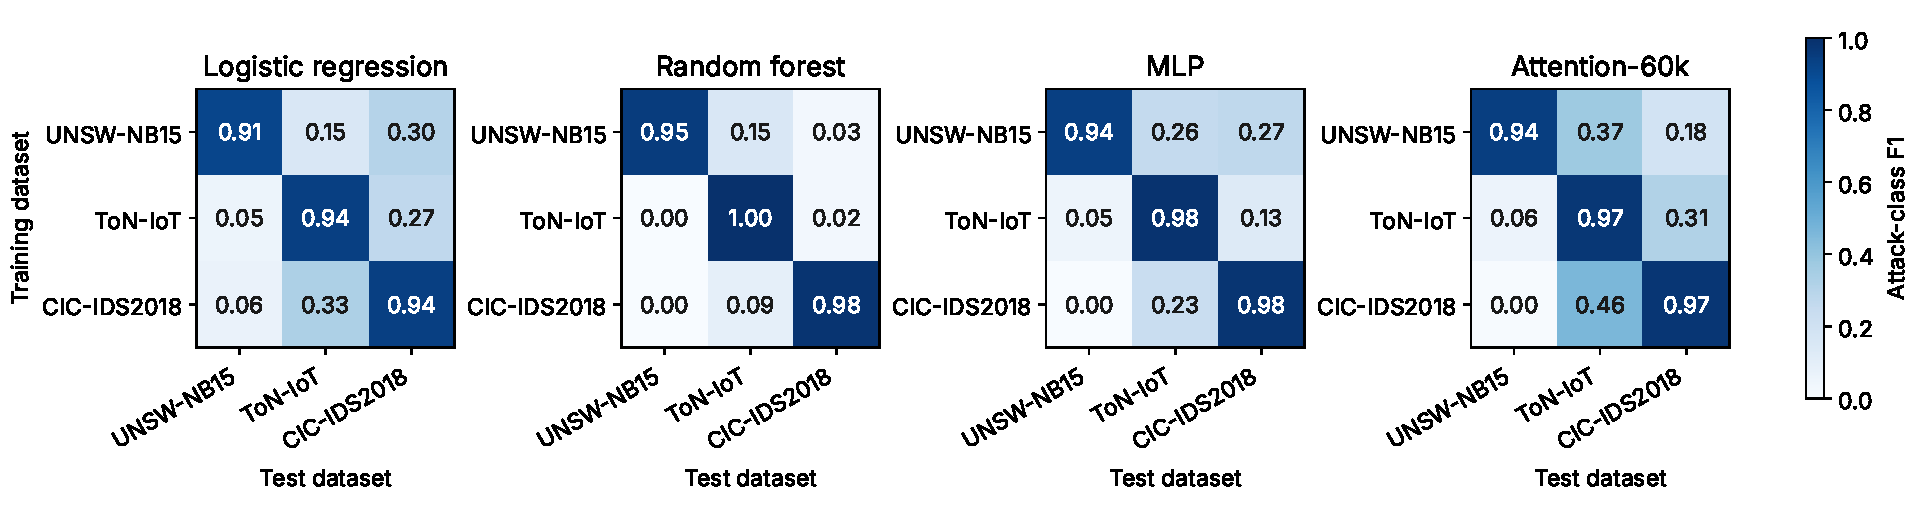
\includegraphics[width=\linewidth]{fig_matrix.pdf}
\caption{Attack-class F1 for every pair of training and test dataset, averaged over three seeds. The diagonal is the in-dataset result. Every off-diagonal cell is a model tested on a network it never saw during training. The attention model was trained on 60,000 flows per source, as described in Section~\ref{sec:method}.}
\label{fig:matrix}
\end{figure*}

\begin{table*}[t]
\centering
\small
\begin{tabular}{lcccccccc}
\toprule
& \multicolumn{3}{c}{F1} & \multicolumn{2}{c}{ROC AUC} & \multicolumn{3}{c}{Cross-dataset} \\
\cmidrule(lr){2-4}\cmidrule(lr){5-6}\cmidrule(lr){7-9}
Model & In-dataset & Cross-dataset & Gap & In-dataset & Cross-dataset & Recall & FPR & Accuracy \\
\midrule
\inputrows tab_summary.tex 
\bottomrule
\end{tabular}
\caption{Summary of single-source transfer. In-dataset values average the three diagonal cells of Figure~\ref{fig:matrix} and cross-dataset values average the six off-diagonal cells, over three seeds. The gap is in-dataset F1 minus cross-dataset F1.}
\label{tab:summary}
\end{table*}

Figure~\ref{fig:matrix} and Table~\ref{tab:summary} show what happens when the test data comes from a different network. Every model falls apart. Averaged over the six cross-dataset pairs, F1 is 0.194 for logistic regression, 0.157 for the MLP, and 0.049 for the random forest. \ATTNCROSS{} No model reaches an F1 above \CROSSMAX{} on any network it was not trained on.

The way the models fail depends on the pair of datasets. Some models flag almost everything. Logistic regression trained on ToN-IoT flags 93.7 percent of the benign flows in UNSW-NB15 and 72.8 percent of the benign flows in CIC-IDS2018. Other models flag almost nothing. The random forest trained on CIC-IDS2018 catches 0 of the attacks in UNSW-NB15, and the random forest trained on ToN-IoT catches 0.3 percent. A deployed detector that floods operators with false alarms and a detector that stays silent during an attack are both useless, and the same models do both depending on where they are moved.

\subsection{Accuracy, F1, and AUC can all mislead}

\FLAGPARA

Accuracy makes several of these failures look fine. The random forest trained on CIC-IDS2018 has an accuracy of 96.0 percent on UNSW-NB15 while detecting no attacks at all, because about 96 percent of UNSW-NB15 is benign and the model labels nearly everything benign. The random forest also has the highest average cross-dataset accuracy in Table~\ref{tab:summary}, at 0.649, even though it has the lowest cross-dataset F1. This is the base rate problem described by Arp \etal \cite{arp2022}, and it is why this project uses attack-class F1 as the main metric.

ROC AUC is not a safe summary either. It does not depend on the threshold, so it could have shown that the models still rank flows correctly and only need a new threshold. That is not what happened. Cross-dataset AUC was at or below 0.5 in 2 of the 6 cross-dataset cells for logistic regression, 3 for the MLP, and 4 for the random forest, with a lowest value of 0.217 for the random forest trained on ToN-IoT and tested on UNSW-NB15. An AUC below 0.5 means the model ranks benign flows as more suspicious than attacks. Recalibrating the threshold on the new network would not fix these models, because what they learned points the wrong way.

\subsection{More complex models do not generalize better}

The ranking of the models flips between the two settings. The random forest is the best model in-dataset, with an average F1 of 0.977 and an average AUC of 0.996. It is the worst model across datasets, with an average cross-dataset AUC of 0.413. Logistic regression is the weakest model in-dataset and has the second smallest gap, 0.736, just behind the attention model discussed next. This supports the hypothesis from the proposal that more flexible models would score higher in-dataset without generalizing better. A model with more capacity can fit the specific patterns of one lab more closely, and those are exactly the patterns that do not carry over.

\ATTNPARA

\subsection{Training on two networks does not close the gap}

\begin{table*}[t]
\centering
\small
\resizebox{\linewidth}{!}{\begin{tabular}{lcccccccc}
\toprule
& \multicolumn{2}{c}{Held out UNSW-NB15} & \multicolumn{2}{c}{Held out ToN-IoT} & \multicolumn{2}{c}{Held out CIC-IDS2018} & \multicolumn{2}{c}{Average} \\
\cmidrule(lr){2-3}\cmidrule(lr){4-5}\cmidrule(lr){6-7}\cmidrule(lr){8-9}
Model & One source & Two sources & One source & Two sources & One source & Two sources & One source & Two sources \\
\midrule
\inputrows tab_multi.tex 
\bottomrule
\end{tabular}}
\caption{Attack-class F1 on a held-out dataset. One source is the average F1 of the two single-source models trained on the other datasets. Two sources is the model trained on both of those datasets combined. \MULTICAPTION}
\label{tab:multi}
\end{table*}

\begin{figure*}[t]
\centering
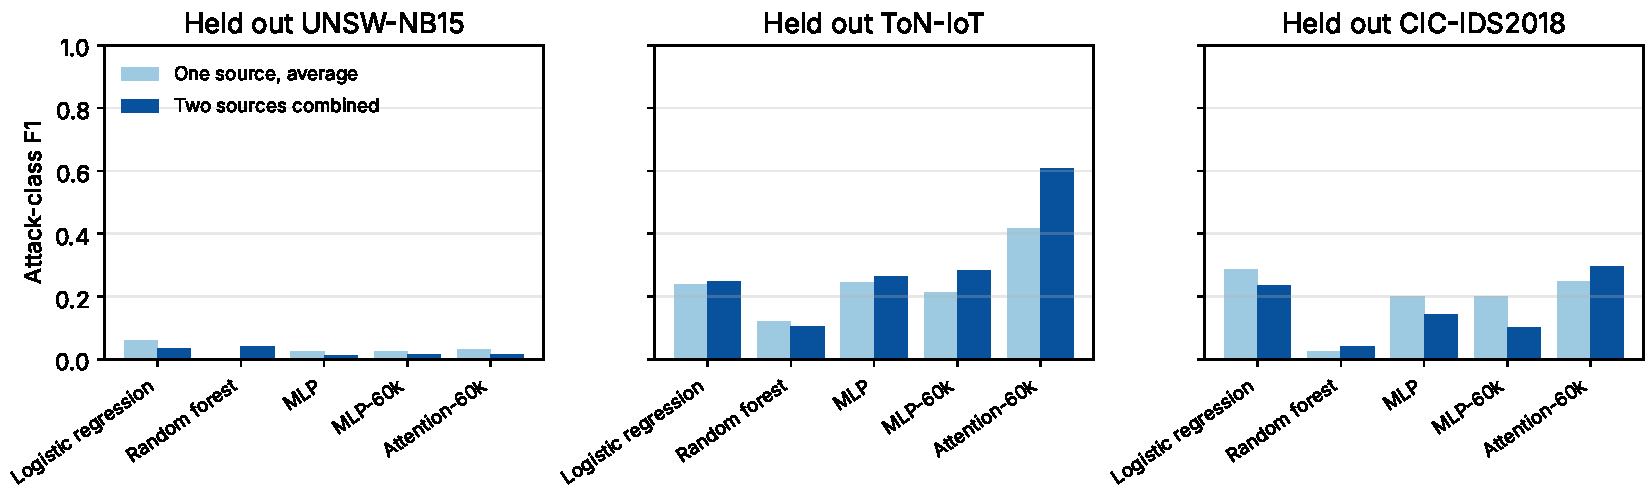
\includegraphics[width=0.9\linewidth]{fig_multi.pdf}
\caption{Held-out F1 with one training source, averaged over the two possible sources, and with both sources combined.}
\label{fig:multi}
\end{figure*}

The proposal expected that training on more than one network would shrink the gap without closing it. Table~\ref{tab:multi} and Figure~\ref{fig:multi} show that it barely shrinks it at all. Averaged over the three held-out datasets, the held-out F1 of logistic regression goes from 0.194 with one source to 0.173 with two, and the MLP goes from 0.157 to 0.139. The random forest goes from 0.049 to 0.061. None of these changes is large enough to matter, and two of them go the wrong way. \MULTIATTN

The reason shows up when the multi-source models are tested on the two networks they were trained on. The random forest still gets an average F1 of 0.976 on those two networks and the MLP gets 0.965, almost the same as their single-source in-dataset scores. Both models are flexible enough to learn a separate rule for each network instead of finding what the attacks have in common. A third network gets neither rule. Logistic regression cannot do this, and its F1 on its own two training networks drops to 0.748. A single linear boundary cannot fit both networks at once, which is more evidence that the networks really are different problems.

\subsection{What the models rely on}
\label{sec:features}

\begin{table*}[t]
\centering
\small
\resizebox{\linewidth}{!}{\begin{tabular}{llllllll}
\toprule
Model & Trained on & First & Drop & Second & Drop & Third & Drop \\
\midrule
\inputrows tab_features.tex
\bottomrule
\end{tabular}}
\caption{The three most important features for each in-dataset model by permutation importance. Drop is the average fall in ROC AUC on the model's own test set when that feature is shuffled.}
\label{tab:features}
\end{table*}

\begin{table}[t]
\centering
\small
\resizebox{\columnwidth}{!}{\begin{tabular}{lll}
\toprule
Dataset & Benign MIN\_TTL & Attack MIN\_TTL \\
\midrule
UNSW-NB15 & 31 in 98.4\% & 254 in 75.2\%, 62 in 24.6\% \\
ToN-IoT & 0 in 84.6\% & 0 in 52.8\%, 64 in 46.1\% \\
CIC-IDS2018 & 0 in 40.7\% & 127 in 61.2\%, 63 in 26.7\% \\
\bottomrule
\end{tabular}}
\caption{Most common MIN\_TTL values in each sample, split by class.}
\label{tab:ttl}
\end{table}

Table~\ref{tab:features} lists the most important features for the random forest and the MLP on each dataset. The two models trained on UNSW-NB15 both rank the TTL features near the top. On ToN-IoT both models depend heavily on L7\_PROTO, the layer 7 protocol ID. Shuffling it alone lowers the random forest's AUC by 0.111. The MLP trained on CIC-IDS2018 leans mostly on TCP\_FLAGS. The random forest's importance values are small in general, because it can usually fall back on another feature that carries the same information when one is shuffled.

The more important point is that the models learn different rules on each network. The Spearman rank correlation between the MLP's feature importance on two different datasets is only between \SPMLPMIN{} and \SPMLPMAX{}, so a feature that matters on one network says little about whether it matters on another. The benign traffic itself is also very different. For each feature, a two-sample Kolmogorov-Smirnov statistic was computed between the benign flows of every pair of datasets. The median feature has an average statistic of \KSMED{}, and \KSSHARE{} percent of the features are above 0.5. Normal traffic on one network does not look like normal traffic on another, which is the diversity problem Sommer and Paxson described \cite{sommer2010}.

The TTL features are the clearest example of a lab artifact. Table~\ref{tab:ttl} shows that 98.4 percent of the benign flows in the UNSW-NB15 sample have a minimum TTL of exactly 31, while almost every attack has a TTL of 254 or 62. TTL depends mostly on the operating system that sent the packet and on how many routers it crossed, so these values describe the machines and layout of the UNSW lab and not the attacks. To check how strong this shortcut is, a single rule that labels a flow as an attack whenever its minimum TTL is not 31 was tested. On the UNSW-NB15 test split this rule gets 100 percent recall, a false positive rate of 1.7 percent, and an F1 of 0.832 without any learning. On ToN-IoT and CIC-IDS2018 the same rule flags every single flow. This is the spurious correlation pitfall from Arp \etal \cite{arp2022}, sitting inside one of the most widely used benchmark datasets.

\subsection{Removing the TTL shortcut}

\begin{table}[t]
\centering
\small
\setlength{\tabcolsep}{4pt}
\resizebox{\columnwidth}{!}{\begin{tabular}{lcccccc}
\toprule
& \multicolumn{2}{c}{UNSW in} & \multicolumn{2}{c}{UNSW out} & \multicolumn{2}{c}{All cross} \\
\cmidrule(lr){2-3}\cmidrule(lr){4-5}\cmidrule(lr){6-7}
Model & TTL & No TTL & TTL & No TTL & TTL & No TTL \\
\midrule
\inputrows tab_ablation.tex
\bottomrule
\end{tabular}}
\caption{Attack-class F1 with and without the two TTL features. UNSW in is trained and tested on UNSW-NB15. UNSW out is trained on UNSW-NB15 and averaged over the other two test sets. All cross averages all six cross-dataset pairs.}
\label{tab:ablation}
\end{table}

\ABLATIONPARA

\subsection{Stability across seeds}

In-dataset results barely change between seeds, with F1 moving by less than 0.01 for every model. Cross-dataset results are much less stable. The random forest trained on UNSW-NB15 and tested on ToN-IoT gets an F1 of 0.077, 0.329, and 0.047 for the three seeds. When the test data looks nothing like the training data, small changes in how the model is built decide which wrong rule it ends up using. This is one more reason a single cross-dataset number should not be trusted on its own.


\section{Conclusions and Future Work}

\subsection{Summary}

This project tested whether machine learning intrusion detectors trained on one network still work on another. They do not. Four model families that all score between \INFMIN{} and \INFMAX{} F1 on their own network drop to between \CROSSMIN{} and \CROSSMAXAVG{} average F1 on networks they were not trained on. The random forest, which is the best model in-dataset, transfers the worst, and its cross-dataset AUC is below 0.5 on average. Training on two networks did not help with the third, because flexible models learned a separate rule for each network. The feature analysis showed that the models depend on different features on each network, and that the TTL features in UNSW-NB15 are a lab artifact that a one-line rule can use to reach an F1 of 0.832. \CONCLABLATION

\subsection{Lessons learned}

The biggest lesson is that an in-dataset score on a lab dataset says very little about how a detector will do anywhere else. Before this project, a random forest with 0.977 F1 would have looked like a finished detector. Moved to a new network, the same model catches almost nothing. Any claim about an intrusion detector should come with at least one test on data from a different source.

The second lesson is to check what a model is actually using. The TTL shortcut was not visible in any score. It only showed up after looking at feature importance and then at the raw values. Without that step it would have been easy to report the UNSW-NB15 results as evidence that the models learned attack behavior.

The third lesson is about metrics. Accuracy rewarded models that detected nothing, and AUC below 0.5 showed that some failures cannot be fixed by moving the threshold. Reporting recall, false positive rate, and F1 on the attack class made the failures obvious right away.

There were also practical lessons. The first MLP runs stopped at a fixed 10 epoch cap while the validation loss was still going down, and they had to be rerun with early stopping. The attention model was too slow to train on the full data on a CPU, so it had to be compared against an MLP trained on the same subsample to keep the comparison fair. Planning for compute limits early would have saved time.

\subsection{Limitations}

The results come from samples of about 300,000 flows per dataset, not the full datasets. Only three datasets were used, and they all share the same NetFlow format, so a different feature format could behave differently. The attention model was trained on 60,000 flows per source, and its multi-source runs used one seed. Every model used a fixed threshold of 0.5. The benign-only autoencoder from the proposal's stretch goal was not built.

\subsection{Future work}

The most practical next step is to see how much labeled data from a new network is needed to recover. Fine-tuning each model on a small number of labeled flows from the target network, for example 100 or 1,000, would show whether a detector can be adapted quickly or has to be retrained from scratch. A second direction is domain adaptation methods that use unlabeled traffic from the new network, since benign traffic is easy to collect even when attacks are not. A third is to remove more network-specific features in a systematic way, by dropping features whose benign distribution changes the most between networks and checking whether cross-dataset results improve. Finally, the benign-only autoencoder from the proposal is still worth testing, since a model that only learns what normal traffic looks like does not depend on which attacks a lab happened to run.

\section*{Code}
The code for data sampling, training, evaluation, and every table and figure in this report is available on GitHub.
\begin{center}\footnotesize\mbox{\GITHUB}\end{center}

{
\small
\bibliographystyle{ieeenat_fullname}
\bibliography{refs}
}

\end{document}
